\documentclass[letterpaper,journal]{IEEEtran}
\usepackage[T1]{fontenc}
\usepackage{amsmath,amssymb,amsfonts,amsthm}
\usepackage{array,booktabs,multirow,threeparttable}
\usepackage{graphicx,cite,url}
\usepackage{stfloats}
\usepackage{placeins}
\usepackage[hidelinks]{hyperref}
\graphicspath{{figures/}}

\newcommand{\method}{CFCMT}
\newcommand{\R}{\mathbb{R}}
\newcommand{\ind}{\mathbf{1}}
\DeclareMathOperator*{\argmin}{arg\,min}
\DeclareMathOperator*{\argmax}{arg\,max}
\DeclareMathOperator{\RMS}{RMS}
\DeclareMathOperator{\clip}{clip}

\newtheorem{proposition}{Proposition}
\newtheorem{theorem}{Theorem}
\newtheorem{lemma}{Lemma}
\newtheorem{remark}{Remark}
\hyphenation{net-work net-works coun-ter-fac-tual pen-e-tra-tion ob-serv-abil-i-ty}

\hypersetup{
  pdftitle={CFCMT: Cross-City Traffic Signal Control Under Sparse Connected-Vehicle Observability via Calibrated Counterfactual Action-Cost Transfer},
  pdfauthor={Yifan Zhang, Liang Zheng, Qifan Zhang, and Haoming Li},
  pdfsubject={IEEE Transactions on Intelligent Transportation Systems}
}

\begin{document}

\title{CFCMT: Cross-City Traffic Signal Control Under Sparse Connected-Vehicle Observability via Calibrated Counterfactual Action-Cost Transfer}

\author{Yifan~Zhang, Liang~Zheng, Qifan~Zhang, and Haoming~Li%
\thanks{Yifan Zhang (e-mail: erzhu419@gmail.com; 204201048@csu.edu.cn) and Liang Zheng (corresponding author; e-mail: zhengliang@csu.edu.cn) are with the School of Traffic and Transportation Engineering, Central South University, Changsha, Hunan, China.}%
\thanks{Qifan Zhang is with the Faculty of Information Technology, Monash University Malaysia, Malaysia (e-mail: zhangqifan0419@gmail.com).}%
\thanks{Haoming Li is with the Department of Transportation Engineering, School of Ocean and Civil Engineering, Shanghai Jiao Tong University, Shanghai, China (e-mail: lihaoming@sjtu.edu.cn).}}

\markboth{IEEE Transactions on Intelligent Transportation Systems}%
{Zhang \MakeLowercase{\textit{et al.}}: CFCMT Under Sparse Connected-Vehicle Observability}

\maketitle

\begin{abstract}
Adaptive traffic signal control in near-term connected-vehicle (CV) deployments must operate without full-lane detector coverage, observing only a sparse fraction of equipped vehicles ($p_{\mathrm{CV}}\approx 10\%$). Under such partial observability, canonical pressure policies collapse due to unobserved human-driven queues, while online deep reinforcement learning (DRL) suffers severe credit-assignment variance and costly target-domain exploration. This paper proposes Causal-Factored Cross-City Model Transfer (\method), a predeployment transfer framework that combines causal partial-CV queue reconstruction, zero-restoration counterfactual action-cost labeling, calibrated pairwise ranking transfer, and a demand-confirmed National Electrical Manufacturers Association (NEMA) maximum-red safety shield. Offline labels are generated via bit-exact native-prefix rollouts ($\text{state\_restores}=0$) over 1-hop causal light cones across six multi-city source domains (411 action groups) and two adaptation seeds per target city. Both source and target models share an identical 78-dimensional endpoint-preserving antisymmetric gradient-boosted pairwise ranker, blended via two-fold cross-validation with an exact fold-to-full root-mean-square (RMS) scale consistency factor $\tau_{\mathrm{cal}}$. Across 1,940 one-hour microscopic SUMO runs spanning three external real-world target cities---Los Angeles, Jinan (three demand regimes), and Salt Lake City (two weekday-peak corridors)---on strictly virgin pre-registered test seeds, few-shot \method\ ($B=6$ target groups) achieves the best three-city equal-weight mean waiting time ($154.43$~s), censoring-free system vehicle-hours ($491.2$~veh-h), and completion rate ($86.1\%$) among 18 non-oracle controllers. At $B=6$, \method\ significantly reduces three-city system vehicle-hours against analytical conservation-reconstructed generalized pressure ($-36.9$~veh-h, exact sign-flip $p=0.0391$), target-only learning ($-161.7$~veh-h, Holm-adjusted $p=0.0234$), within-group label-permuted source placebos ($-253.5$~veh-h, Holm $p=0.0234$), and sensor-matched FRAP/MPLight Double-DQN baselines ($-224.0$ to $-406.6$~veh-h, Holm $p=0.0234$), while generalizing without retraining across $p_{\mathrm{CV}}\in\{5\%,10\%,20\%,50\%,100\%\}$.
\end{abstract}

\begin{IEEEkeywords}
Connected vehicles, partial observability, cross-city transfer learning, counterfactual action-cost ranking, traffic signal control, intelligent transportation systems.
\end{IEEEkeywords}

\section{Introduction}
\label{sec:intro}

\IEEEPARstart{U}{rban} traffic signal control increasingly leverages trajectory telemetry broadcast by connected vehicles (CVs) via vehicle-to-infrastructure (V2I) communication to eliminate the installation and maintenance costs of dense inductive-loop or radar detectors \cite{feng2015realtime,tiaprasert2015queue,zhao2022maximum}. However, fleet renewal is gradual: throughout the foreseeable transitional era, CV market penetration rates remain sparse ($p_{\mathrm{CV}}\in[5\%,20\%]$), leaving 80--95\% of approaching human-driven vehicles (HDVs) directly unobservable \cite{zhang2021partial,mo2022cvlight}.

When full-lane vehicle counts are available ($p_{\mathrm{CV}}=100\%$), analytical pressure controllers such as MaxPressure (MP) \cite{varaiya2013maxpressure} and generalized pressure (GP) achieve strong throughput with zero site-specific training, leaving minimal headroom for learned policies. Under realistic $10\%$ CV observability, by contrast, naive pressure heuristics see empty approaches whenever all waiting vehicles in a queue happen to be unequipped HDVs. This ``invisible-queue starvation'' causes premature phase holds on low-demand movements, downstream arterial spillback, and severe gridlock. Analytical shockwave and arrival-conservation estimators \cite{liu2009realtime,tiaprasert2015queue} partially mitigate instantaneous blindness by tracking red-phase CV halting tails and historical CV arrival rates, yet they remain myopic point-estimate heuristics: they ignore estimation variance under sparse sampling, quadratic delay growth of unequipped arrivals during prolonged red intervals, clearance switching losses, and 1-hop downstream spillback coupling.

Learning-based and transferable controllers offer a natural avenue to capture these nonlinear partial-observability dynamics across cities \cite{wei2019presslight,zheng2019frap,chen2020thousandlights,zang2020metalight,jiang2024gesa,jiang2024xlight,sun2024crosslight}, but face four fundamental methodological hurdles:
\begin{enumerate}
    \item \textit{Credit-Assignment Variance Under Sparse Sensing:} Online deep reinforcement learning (DRL) agents trained on partial-CV pressure rewards experience high temporal-difference variance when reward signals themselves depend on noisy $10\%$ probe observations, requiring tens of hours of unsafe online exploration per city \cite{zhang2021partial,mo2022cvlight}.
    \item \textit{Snapshot-Restoration Artifacts in Counterfactual Labeling:} Supervised counterfactual action-cost methods often rely on simulator \texttt{saveState}/\texttt{loadState} snapshots, which can introduce subtle car-following state or signal-executor discrepancies across branches.
    \item \textit{Cross-Validation Scale Shift and Architecture Confounding:} Prior transfer evaluations frequently compare heterogeneous source and target model capacities, or tune blending weights via $K$-fold cross-validation without correcting for the systematic amplitude expansion between half-sample fold predictors and full-sample deployed target tree ensembles.
    \item \textit{Starvation vs.\ False-Trigger Trade-Off in Multi-Phase Rings:} Under sparse CV arrivals, bounding maximum red time prevents unequipped-vehicle starvation on two- and four-phase arterials, but naive fixed red caps falsely trigger on uncalled left-turn pockets in eight-phase NEMA dual-ring intersections.
\end{enumerate}

To resolve these challenges, we develop Causal-Factored Cross-City Model Transfer (\method) for sparse-CV traffic signal control (Fig.~\ref{fig:framework_overview}). Rather than bootstrapping noisy temporal-difference values online, \method\ constructs matched short-horizon counterfactual action groups using bit-exact native-prefix simulator rollouts ($\text{state\_restores}=0$) verified by cryptographic pre-branch state fingerprints. Every experimental arm shares an identical 78-dimensional endpoint-preserving antisymmetric pairwise ranker conditioned strictly on causal partial-CV statistics, combined via scale-consistent cross-validation and shielded online by a two-clause demand-confirmed NEMA maximum-red rule.

The primary contributions of this work are fourfold:
\begin{enumerate}
    \item \textit{Non-Leaking Causal Partial-CV Formulation and Zero-Restoration Counterfactuals:} We formalize strict trip-persistent CV sensing ($p_{\mathrm{CV}}=10\%$) with shockwave and conservation queue reconstruction, and introduce native-prefix 1-hop light-cone counterfactual labeling with zero simulator state restores and zero pre-branch fingerprint mismatches across 539 multi-city action groups.
    \item \textit{Architecture-Matched Endpoint-Antisymmetric Transfer with RMS Scale Calibration:} We design a 78-dimensional pairwise action-cost ranker $[x_g,\phi_i-\phi_j,\tfrac{1}{2}(\phi_i+\phi_j)]$ with independent-group leaf regularization and prove exact Borda ranking recovery, cross-validation RMS scale consistency ($\tau_{\mathrm{cal}}$), and single-step regret bounds.
    \item \textit{Two-Clause Demand-Confirmed NEMA Maximum-Red Shield:} We derive a cycle-proportional safety shield combining a confirmed-CV waiting cap with an arrival-flow-confirmed drought cap, proving analytical immunity against false triggers on uncalled dual-ring phases under exponential prior decay.
    \item \textit{Pre-Registered Multi-City Virgin-Seed Evaluation:} Across 1,940 one-hour closed-loop runs on Los Angeles, Jinan (repaired zero-conflict network across three demand levels), and Salt Lake City (two weekday-peak corridors), we demonstrate statistically significant reductions in system vehicle-hours and waiting time over analytical conservation-pressure baselines, architecture-matched target-only and label-permuted source-placebo controls, and sensor-matched FRAP/MPLight Double-DQN baselines, plus zero-retraining generalization across $p_{\mathrm{CV}}\in[5\%,100\%]$.
\end{enumerate}

\section{Related Work}
\label{sec:related}

\subsection{Queue Estimation and Signal Control With Connected Vehicles}
Early V2I signal control studies reconstructed approach queues from probe stopping positions and shockwave theory. Liu \emph{et~al.} \cite{liu2009realtime} identified real-time queue tails from shockwave break points during red intervals, while Tiaprasert \emph{et~al.} \cite{tiaprasert2015queue} formulated queue estimation under pretimed and actuated control at sparse CV penetrations. Feng \emph{et~al.} \cite{feng2015realtime} coupled shockwave-estimated unequipped arrivals with bi-level phase allocation, and Zhao \emph{et~al.} \cite{zhao2022maximum} developed maximum-likelihood penetration and queue distribution estimators from probe trajectories. More recently, DRL controllers such as Zhang \emph{et~al.} \cite{zhang2021partial} and CVLight \cite{mo2022cvlight} trained decentralized policies directly from partial CV detections. However, purely target-trained CV-DRL requires extensive target-network interaction, whereas analytical shockwave-pressure rules degrade sharply on coordinated arterials at $p_{\mathrm{CV}}\le 10\%$. Our work bridges both paradigms by embedding causal shockwave, conservation, and quadratic hidden-delay statistics into a cross-city counterfactual ranker that adapts with as few as $B\in\{0,6\}$ target states.

\subsection{Pressure-Based and Phase-Competition DRL Controllers}
Varaiya \cite{varaiya2013maxpressure} established queue stability of canonical MP under full queue observability. In DRL, PressLight \cite{wei2019presslight} aligned arterial rewards with pressure differentials, FRAP \cite{zheng2019frap} introduced permutation- and rotation-invariant phase competition across heterogeneous intersection geometries, MPLight \cite{chen2020thousandlights} scaled FRAP with pressure features to city-wide grids, and CoLight \cite{wei2019colight} incorporated graph attention over 1-hop neighbors. In our evaluation, we implement both analytical partial-CV pressure hierarchy baselines (Observed MP/PP/GP, Shockwave-GP, Conservation-GP, and MaxRed-Conservation-GP) and sensor-matched FRAP/MPLight Double-DQN agents over the exact same 10\% CV observer and physical clearance executor.

\subsection{Cross-City Transfer and Causal Representation Learning}
Transferable signal control frameworks aim to amortize simulation experience across cities. MetaLight \cite{zang2020metalight} applied value-based gradient meta-learning, GESA \cite{jiang2024gesa} standardized scenario-agnostic state-action interfaces across heterogeneous intersections, X-Light \cite{jiang2024xlight} trained transformer-on-transformer meta-policies across multi-city trajectories, and CrossLight \cite{sun2024crosslight} combined offline source pretraining with online target fine-tuning. From a causal representation perspective \cite{bengio2019meta,scholkopf2021causal,feng2022factored}, local traffic discharge mechanics---saturation flow, yellow/all-red clearance loss, shockwave propagation, and hidden unequipped arrival accumulation---obey invariant physical laws across cities, whereas background demand levels and phase-ring multiplex ratios shift across domains. \method\ isolates invariant action-cost contrasts by differencing matched native-prefix branches within each state and calibrating structural source priors via scale-consistent cross-validation.

\begin{figure*}[!t]
\centering
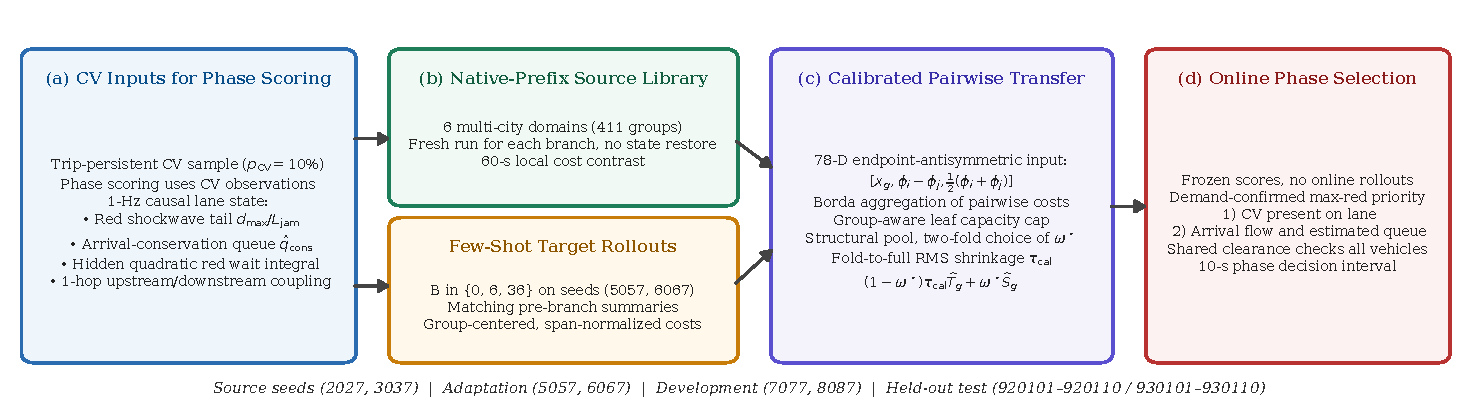
\includegraphics[width=\textwidth]{fig1_framework.pdf}
\caption{Architecture of \method\ under sparse connected-vehicle partial observability ($p_{\mathrm{CV}}=10\%$). (a) A causal 1-Hz observer tracks only deterministically hashed CVs, reconstructing shockwave and arrival-conservation queues without querying unequipped HDVs. (b) Native-prefix rollouts ($\text{state\_restores}=0$) generate bit-exact counterfactual 1-hop light-cone delay contrasts across six multi-city source domains and few-shot target adaptation seeds. (c) Architecture-matched 78-D endpoint-antisymmetric gradient-boosted rankers are blended using two-fold cross-validation with exact fold-to-full RMS parity calibration $\tau_{\mathrm{cal}}$. (d) Online control executes frozen scores under a two-clause demand-confirmed NEMA maximum-red shield and shared physical clearance executor.}
\label{fig:framework_overview}
\end{figure*}

\section{Problem Formulation and Partial-CV Sensing}
\label{sec:problem}

\subsection{Strict Non-Leaking Partial-CV Observation Model}
Consider an urban road network comprising signalized intersections $\mathcal{I}$, controlled incoming lanes $\mathcal{L}_{\mathrm{in}}$, and immediate outgoing lanes $\mathcal{L}_{\mathrm{out}}$. Each entering vehicle $v$ is independently and persistently equipped with V2I telemetry at market penetration rate $p_{\mathrm{CV}}\in(0,1]$ via a deterministic cryptographic hash:
\begin{equation}
  \mathrm{CV}(v;\xi,p_{\mathrm{CV}}) = \ind\!\left\{\frac{\operatorname{uint64}(\operatorname{blake2b}(\xi \,\|\, v))}{2^{64}} < p_{\mathrm{CV}}\right\},
  \label{eq:cv_hash}
\end{equation}
where $\xi$ is the episode seed. Drawing equipment status via \eqref{eq:cv_hash} consumes zero simulator random numbers and guarantees trip-level persistence without trajectory ID spoofing. Unequipped HDVs ($\mathrm{CV}(v)=0$) are strictly invisible: their positions, speeds, waiting times, and halting states are never queried during feature extraction, reward computation, or online control. To enforce this invariant architecturally, our feature extractor does not accept the simulator handle as an argument.

At 1-Hz step $t$, let $\mathcal{V}_{\ell}^{\mathrm{CV}}(t)$ denote equipped CVs on lane $\ell$ of length $L_\ell$ and speed limit $v_{\max,\ell}$. The observer records raw CV count $n_\ell^{\mathrm{CV}}(t)$, halted CV count $h_\ell^{\mathrm{CV}}(t)$ ($v < 0.1$~m/s), slow CV count ($v < 2.0$~m/s), CV occupancy percentage $o_\ell^{\mathrm{CV}}(t)$, stopbar distance of the farthest halted CV $d_{\max,\ell}^{\mathrm{CV}}(t)$, cumulative CV halt wait $W_\ell^{\mathrm{CV}}(t)$, elapsed red/green durations $(\tau_{\mathrm{red},\ell}(t),\tau_{\mathrm{green},\ell}(t))$, and newly observed CV arrivals $\Delta A_\ell^{\mathrm{CV}}(t)$ deduplicated per lane traversal.

From these strictly observable quantities, each lane maintains two causal arrival-rate exponential moving averages ($\tau_w\in\{60,300\}$~s, initialized at conservative prior $\lambda_0=0.04$~veh/s):
\begin{equation}
\begin{split}
  \hat{\lambda}_{\ell,\tau_w}(t) &= e^{-\Delta t_s/\tau_w}\hat{\lambda}_{\ell,\tau_w}(t-\Delta t_s)\\
  &\quad + \bigl(1 - e^{-\Delta t_s/\tau_w}\bigr)\frac{\Delta A_\ell^{\mathrm{CV}}(t)}{p_{\mathrm{CV}}\Delta t_s},
\end{split}
  \label{eq:ema_arrival}
\end{equation}
where $\Delta t_s=1$~s. Letting $d_{\max,\ell}^{\mathrm{red}}(t)$ track the maximum CV halt distance observed during the current red window (decaying at saturation speed during green), the shockwave queue estimate \cite{liu2009realtime} and arrival-conservation queue estimate are updated as:
\begin{align}
  \hat{q}_{\mathrm{sw},\ell}(t) &= \min\!\left(\frac{L_\ell}{L_{\mathrm{jam}}},\; \max\!\left(\frac{h_\ell^{\mathrm{CV}}(t)}{p_{\mathrm{CV}}},\; \frac{d_{\max,\ell}^{\mathrm{red}}(t)}{L_{\mathrm{jam}}}\right)\right), \label{eq:q_sw}\\
  \tilde{q}_{\mathrm{cons},\ell}(t) &= \hat{q}_{\mathrm{cons},\ell}(t-\Delta t_s) + \frac{\Delta A_\ell^{\mathrm{CV}}(t)}{\max(p_{\mathrm{CV}},0.25)} \nonumber\\
  &\quad + (1-p_{\mathrm{CV}})\hat{\lambda}_{\ell,300}(t)\Delta t_s - \ind_{\mathrm{green},\ell}^{\mathrm{eff}}(t)\,s_{\mathrm{sat}}\Delta t_s, \label{eq:q_cons_raw}\\
  \hat{q}_{\mathrm{cons},\ell}(t) &= \clip\!\Bigl(\max\bigl(\tilde{q}_{\mathrm{cons},\ell}(t),\, h_\ell^{\mathrm{CV}}(t),\nonumber\\
  &\qquad\qquad\quad 0.85\hat{q}_{\mathrm{sw},\ell}(t)\bigr),\, 0,\, L_\ell/L_{\mathrm{jam}}\Bigr), \label{eq:q_cons}
\end{align}
where $L_{\mathrm{jam}}=7.5$~m is jam spacing, $s_{\mathrm{sat}}=0.45$~veh/s is per-lane saturation discharge after a 2-s startup lost time ($\ind_{\mathrm{green},\ell}^{\mathrm{eff}}(t)=\ind\{\tau_{\mathrm{green},\ell}(t)>2\}$), and single-arrival spikes in \eqref{eq:q_cons_raw} are damped by $\max(p_{\mathrm{CV}},0.25)$ while preserving unbiased long-run flow via $\hat{\lambda}_{\ell,300}$.

\subsection{Zero-Restoration Native-Prefix Counterfactual Labeling}
At discrete control epochs $\Delta t=10$~s, each intersection $i\in\mathcal{I}$ chooses a requested green phase $a\in\mathcal{A}(s_g)$ through a shared physical executor enforcing minimum green, yellow, and all-red clearance intervals \cite{lopez2018microscopic}. To eliminate all \texttt{saveState}/\texttt{loadState} snapshot-restoration artifacts, we generate matched counterfactual action groups $g$ via \emph{native-prefix replay} ($\text{state\_restores}=0$). Given seed $\xi$, decision epoch $t_g$, and focal intersection $i_g$ with $K_g=|\mathcal{A}_g|\ge 2$ feasible phases, each candidate branch $a\in\mathcal{A}_g$ replays the identical deterministic behavior policy from $t=0$ to $t_g$. At $t_g$, we compute a cryptographic fingerprint over simulation time, current green phase, elapsed green, and CV observations; across all 539 source and target groups in this study, pre-branch fingerprint mismatches equal identically zero.

Over the subsequent $H=60$-s horizon ($\tau\in\{1,\dots,60\}$), focal intersection $i_g$ executes candidate $a$ for $10$~s and follows Conservation-GP for $50$~s, while non-focal intersections follow Conservation-GP throughout. Rather than summing noisy city-wide queues unrelated to $i_g$, we integrate halted-vehicle delay over the 1-hop causal light cone $\mathcal{L}_1(i_g)$ (incoming lanes of $i_g$, immediate outgoing lanes, and incoming lanes of 1-hop downstream neighbors):
\begin{equation}
\begin{split}
  Y_g(a) = \frac{1}{H\,|\mathcal{L}_1(i_g)|}\sum_{\tau=1}^{H}\Biggl(&\sum_{\ell\in\mathcal{L}_1(i_g)} N_{\mathrm{halted},\ell}(\tau)\\
  &+ 0.25\,N_{\mathrm{pending}}(\tau)\Biggr).
\end{split}
  \label{eq:lightcone_cost}
\end{equation}
Note that ground-truth halting counts $N_{\mathrm{halted},\ell}(\tau)$ in \eqref{eq:lightcone_cost} are used \emph{solely as offline simulator training targets} on predeployment source seeds $(2027,3037)$ and two target adaptation seeds $(5057,6067)$---analogous to simulator-based offline RL rewards---and are never accessed during online control. With soft-floored group span $\sigma_g = \max\{\max_a Y_g(a)-\min_a Y_g(a),\,\sigma_{\min}\}$ ($\sigma_{\min}=0.15$), the centered normalized branch cost and single-step normalized action regret are:
\begin{align}
  z_g(a) &= \frac{Y_g(a)-\frac{1}{K_g}\sum_{a'\in\mathcal{A}_g}Y_g(a')}{\sigma_g},\nonumber\\
  R_g(a) &= \frac{Y_g(a)-\min_{a'\in\mathcal{A}_g}Y_g(a')}{\sigma_g}.
  \label{eq:norm_cost}
\end{align}

\section{Methodology: The CFCMT Framework}
\label{sec:method}

\subsection{Physics-Informed Partial-CV State--Action Representation}
For any decision state $g$ with feasible phases $\mathcal{A}_g=(a_1,\dots,a_{K_g})$, we extract a geometry-invariant state vector $x_g\in\R^{18}$ and per-phase descriptor $\phi_g(a_i)\in\R^{30}$ across \emph{all} controlled incoming lanes of $i_g$ (preserving shared-upstream right-turn lanes so that 33\% of approach CV observations are not lost on multi-lane approaches). Specifically, $x_g$ encodes inverse-$p_{\mathrm{CV}}$-scaled CV halted and total densities, mean and maximum shockwave and conservation queues, mean and maximum normalized red ages, current green age, 60-s and 300-s arrival rates, maximum CV wait, fraction of lanes with active CVs, normalized candidate count $K_g/8$ and lane count $|\mathcal{L}_{\mathrm{in}}(i_g)|/16$, 1-hop upstream and downstream mean conservation queues, and $p_{\mathrm{CV}}$ itself.

For each candidate phase $a_i\in\mathcal{A}_g$ serving green lane set $\mathcal{G}(a_i)$ while holding $\mathcal{R}(a_i)=\mathcal{L}_{\mathrm{in}}(i_g)\setminus\mathcal{G}(a_i)$ red, $\phi_g(a_i)\in\R^{30}$ captures: (i) relative Conservation-GP, Shockwave-GP, and Observed-GP pressures normalized to $[-0.5,1.0]$; (ii) expected total waiting-time share combining observed CVs with the quadratic unequipped red-arrival delay integral
\begin{equation}
  \widehat{W}_{\mathrm{hid}}(a_i) = \sum_{\ell\in\mathcal{G}(a_i)}\left[\frac{W_\ell^{\mathrm{CV}}}{p_{\mathrm{CV}}} + \frac{1}{2}(1-p_{\mathrm{CV}})\hat{\lambda}_{\ell,300}\tau_{\mathrm{red},\ell}^2\right];
  \label{eq:quad_wait}
\end{equation}
(iii) green-movement flow share, lane ratio, CV densities, shockwave/conservation queues, spillback fraction, speed ratio, and 10-s serviceable discharge accounting for projected clearance loss $c_{\mathrm{clr}}(a_i)$ and downstream occupancy; (iv) competing red-movement conservation queue, maximum red age, and quadratic red wait; and (v) downstream scaled occupancy, downstream shockwave queue, switching indicator, normalized clearance time, and continuation green age.

\subsection{Endpoint-Preserving Antisymmetric Pairwise Ranker}
To guarantee strict architectural parity across zero-shot, target-only, placebo, pooled, and transfer controllers, every learned arm uses the exact same \texttt{EndpointAntisymmetricActionRanker}. In partial-CV traffic control, pure feature differences $\phi_g(a_i)-\phi_g(a_j)$ lose absolute congestion context: a 2-vehicle queue differential has negligible delay impact under free flow but triggers upstream gridlock near spillback saturation. For each unordered pair $(a_i,a_j)$ ($i<j$), we construct the 78-dimensional endpoint-preserving pairwise vector:
\begin{equation}
  u_{gij} = \bigl[\, x_g,\; \phi_g(a_i)-\phi_g(a_j),\; \tfrac{1}{2}\bigl(\phi_g(a_i)+\phi_g(a_j)\bigr) \,\bigr] \in \R^{78},
  \label{eq:pair_vec}
\end{equation}
paired with target $t_{gij}=z_g(a_i)-z_g(a_j)$ and its antisymmetric reflection $u_{gji}=[x_g,\phi_g(a_j)-\phi_g(a_i),\tfrac{1}{2}(\phi_g(a_i)+\phi_g(a_j))]$ with target $-t_{gij}$. Each training domain $d$ receives equal total mass $w_d$ balanced across groups and pairs, weighted by contrast importance $\clip(\sigma_g/\sigma_{\min},0.25,4.0)$.

Because an $8$-phase intersection generates $2\binom{8}{2}=56$ correlated pairwise rows from a \emph{single} independent traffic state, sizing gradient-boosted regression trees \cite{friedman2001greedy,pedregosa2011scikit} solely by pairwise row count causes severe memorization at small target budgets ($B=6$). Letting $N_g$ denote the number of independent multi-action groups, we enforce group-aware leaf regularization:
\begin{equation}
  L_{\max}(N_g) = \begin{cases}
    4, & \text{if } N_g \le 12,\\
    15, & \text{if } N_g > 12,
  \end{cases}
  \label{eq:leaf_cap}
\end{equation}
with learning rate $0.05$, $120$ boosting iterations, minimum leaf samples $\min(20,\max(6,\lfloor N_{\mathrm{rows}}/6\rfloor))$, and $L_2$ penalty $15.0$ across all arms. At inference, let $f_\psi:\R^{78}\to\R$ be the fitted regressor. Exact antisymmetry and Borda cost aggregation yield:
\begin{align}
  \widehat{\delta}_{gij} &= \tfrac{1}{2}\bigl[f_\psi(u_{gij}) - f_\psi(u_{gji})\bigr], \label{eq:antisym}\\
  P_g(a_i) &= \frac{1}{K_g - 1}\sum_{j\ne i}\widehat{\delta}_{gij}, \label{eq:borda}
\end{align}
where lower $P_g(a_i)$ indicates lower predicted 60-s light-cone delay.

\subsection{Structural Routing and Scale-Consistent Blending}
Source domains are organized into structural pools reflecting signal phasing geometry: $\mathcal{P}_{\mathrm{real}}$ (all real-world cities: Hangzhou homogeneous and Gudang heterogeneous grids, Atlanta arterial, Cologne, and Ingolstadt) for corridors containing two- to four-phase intersections ($\min_g K_g < 6$), and $\mathcal{P}_{\mathrm{grid}}$ (multi-phase urban grids) when all target intersections operate high-cardinality dual-ring plans ($\min_g K_g \ge 6$).

Given $B$ target adaptation groups partitioned by adaptation seed into $\mathcal{D}_0$ ($\xi=5057$) and $\mathcal{D}_1$ ($\xi=6067$), we fit fold predictors $\widehat{T}^{(-0)}$ on $\mathcal{D}_1$ and $\widehat{T}^{(-1)}$ on $\mathcal{D}_0$ to obtain out-of-fold (OOF) target scores $\widehat{T}_g^{\mathrm{OOF}}$. Across candidate pool $p$ and $\omega\in\Omega=\{0.08,0.18,0.25,0.50,0.75,0.90,1.00\}$, we select $(p^\star,\omega^\star)$ minimizing OOF mean normalized regret, breaking discrete step-function ties via smooth Boltzmann expected regret ($\tau_B=0.08$):
\begin{equation}
  \mathcal{R}_{\tau_B}(\widehat{S}) = \frac{1}{|\mathcal{D}_{\mathrm{adapt}}|}\sum_{g}\sum_{a\in\mathcal{A}_g}\frac{\exp(-\widehat{S}_g(a)/\tau_B)}{\sum_{a'}\exp(-\widehat{S}_g(a')/\tau_B)}R_g(a).
  \label{eq:boltzmann}
\end{equation}

Crucially, when the final target ranker $\widehat{T}^{\mathrm{full}}$ is refitted on all $B=|\mathcal{D}_0\cup\mathcal{D}_1|$ groups, doubling sample size increases leaf resolution and reduces shrinkage, expanding $\RMS(\widehat{T}^{\mathrm{full}}) > \RMS(\widehat{T}^{\mathrm{OOF}})$ (by up to $1.33\times$ in our audits) while the source predictor $\widehat{S}_{p^\star}$ remains unchanged. Deploying uncalibrated $(1-\omega^\star)\widehat{T}^{\mathrm{full}}+\omega^\star\widehat{S}_{p^\star}$ silently distorts the cross-validated signal ratio. We therefore compute the adaptation-set fold-to-full scale factor:
\begin{equation}
  \tau_{\mathrm{cal}} = \min\!\left(1,\; \frac{\RMS_{g\in\mathcal{D}_{\mathrm{adapt}}}(\widehat{T}_g^{\mathrm{OOF}})}{\max\bigl(\RMS_{g\in\mathcal{D}_{\mathrm{adapt}}}(\widehat{T}_g^{\mathrm{full}}),\,10^{-9}\bigr)}\right),
  \label{eq:tau_cal}
\end{equation}
and deploy the calibrated convex ranker:
\begin{equation}
  F_g(a) = (1-\omega^\star)\,\tau_{\mathrm{cal}}\,\widehat{T}_g^{\mathrm{full}}(a) + \omega^\star\,\widehat{S}_{p^\star,g}(a).
  \label{eq:calibrated_blend}
\end{equation}
Calculating $\tau_{\mathrm{cal}}$ strictly on $\mathcal{D}_{\mathrm{adapt}}$ preserves zero test leakage and applies identically to \method, Source-Placebo, and Pool-All arms.

\subsection{Two-Clause Demand-Confirmed NEMA Maximum-Red Shield}
Under $p_{\mathrm{CV}}=10\%$, nine out of ten approaching vehicles are invisible; if a side-street queue contains exclusively unequipped HDVs, any unconstrained controller can starve that movement indefinitely. Conversely, a naive fixed maximum-red cap (e.g., $110$~s) triggers constantly on empty left-turn pockets in 8-phase dual-ring intersections, destroying arterial progression. Let $M_i = |\mathcal{L}_{\mathrm{in}}(i)|/\max(1,\overline{g}_i)$ denote the intersection's phase-multiplexing ratio (ratio of total incoming lanes to average green lanes per phase; $M_i\approx 2.0$ on 2-phase arterials and $M_i\approx 6.0$ on 8-phase dual-ring grids). Lane $\ell$ is flagged as \emph{overdue} if and only if it satisfies either of two demand-confirmed clauses:
\begin{align}
  \mathcal{C}_1(\ell) &: \tau_{\mathrm{red},\ell} \ge \max(115,\,70M_i-25) \nonumber\\
  &\quad \wedge\; \bigl(h_\ell^{\mathrm{CV}}\ge 1 \vee n_\ell^{\mathrm{CV}}\ge 1\bigr), \label{eq:clause1}\\
  \mathcal{C}_2(\ell) &: \tau_{\mathrm{red},\ell} \ge \clip(75M_i,\,140,\,310) \;\wedge\; \hat{\lambda}_{\ell,300}\ge 0.020 \nonumber\\
  &\quad \wedge\; \max(\hat{q}_{\mathrm{sw},\ell},\hat{q}_{\mathrm{cons},\ell}) \ge 2.0. \label{eq:clause2}
\end{align}
Let $\mathcal{O}_g=\{\ell\in\mathcal{L}_{\mathrm{in}}(i_g):\mathcal{C}_1(\ell)\vee\mathcal{C}_2(\ell)\}$ be overdue lanes and $\tau_{\mathrm{red}}^{\star}=\max_{\ell\in\mathcal{O}_g}\tau_{\mathrm{red},\ell}$. When $\mathcal{O}_g\ne\emptyset$, online phase selection restricts $\mathcal{A}_g$ to the relieving subset $\mathcal{A}_g^{\mathrm{safe}}=\{a\in\mathcal{A}_g:\exists\,\ell\in\mathcal{G}(a)\cap\mathcal{O}_g \text{ s.t. } \tau_{\mathrm{red},\ell}\ge\tau_{\mathrm{red}}^{\star}-5\}$ and minimizes $F_g(a)$ over $a\in\mathcal{A}_g^{\mathrm{safe}}$.

\subsection{Theoretical Properties}
Proofs of Propositions~\ref{prop:offset}--\ref{prop:maxred} are provided in Appendix~\ref{app:proofs}.

\begin{proposition}[Common-Offset Cancellation]
\label{prop:offset}
If $Y_g(a)=b_g+\mu_g(a)+e_g(a)$ for an arbitrary state-dependent congestion baseline $b_g$ common to all $a\in\mathcal{A}_g$, then $z_g(a)$ in \eqref{eq:norm_cost} and $t_{gij}=z_g(a_i)-z_g(a_j)$ are strictly invariant to $b_g$, and invariant to positive rescaling whenever $\max_a Y_g(a)-\min_a Y_g(a)\ge\sigma_{\min}$.
\end{proposition}

\begin{proposition}[Exact Borda Recovery and Endpoint Expressivity]
\label{prop:expressivity}
The pairwise score in \eqref{eq:antisym}--\eqref{eq:borda} satisfies $\widehat{\delta}_{gij}=-\widehat{\delta}_{gji}$ and $\sum_{a\in\mathcal{A}_g}P_g(a)=0$. If $\widehat{\delta}_{gij}=z_g(a_i)-z_g(a_j)$ for all $i\ne j$, then $P_g(a_i)=\frac{K_g}{K_g-1}z_g(a_i)$, recovering the exact action ordering and ties. Moreover, there exist quadratic congestion cost functions $z_g(a)=\phi_g(a)^\top Q\phi_g(a)$ ($Q\succ 0$) for which no function of $[\,x_g,\phi_g(a_i)-\phi_g(a_j)\,]$ alone can represent $z_g(a_i)-z_g(a_j)$, whereas $u_{gij}$ in \eqref{eq:pair_vec} represents $z_g(a_i)-z_g(a_j)=2(\phi_g(a_i)-\phi_g(a_j))^\top Q\,\bigl[\tfrac{1}{2}(\phi_g(a_i)+\phi_g(a_j))\bigr]$ exactly.
\end{proposition}

\begin{proposition}[RMS Scale Consistency and Regret Bound]
\label{prop:regret}
Under $\tau_{\mathrm{cal}}$ in \eqref{eq:tau_cal}, whenever $\RMS(\widehat{T}^{\mathrm{full}})\ge\RMS(\widehat{T}^{\mathrm{OOF}})$, the deployed target component $\tau_{\mathrm{cal}}\widehat{T}^{\mathrm{full}}$ has identical adaptation-set $\ell_2$ dispersion to $\widehat{T}^{\mathrm{OOF}}$. Furthermore, for $\widehat{a}_g\in\argmin_{a\in\mathcal{A}_g}F_g(a)$ and $\tilde{z}_g=\frac{K_g}{K_g-1}z_g$, single-step normalized regret satisfies:
\begin{equation}
\begin{split}
  R_g(\widehat{a}_g) \le \frac{2(K_g-1)}{K_g}\Bigl[&(1-\omega^\star)\|\tau_{\mathrm{cal}}\widehat{T}_g^{\mathrm{full}}-\tilde{z}_g\|_\infty\\
  &+ \omega^\star\|\widehat{S}_{p^\star,g}-\tilde{z}_g\|_\infty\Bigr].
\end{split}
  \label{eq:regret_bound}
\end{equation}
\end{proposition}

\begin{proposition}[Dead-Pocket Immunity of Two-Clause Max-Red]
\label{prop:maxred}
Consider an uncalled turning lane $\ell$ receiving zero vehicle arrivals ($\Delta A_\ell^{\mathrm{CV}}(t)\equiv 0$ and $n_\ell^{\mathrm{CV}}(t)\equiv 0$) from $t=0$ under prior initialization $\hat{\lambda}_{\ell,300}(0)=\lambda_0=0.04$~veh/s. For every intersection with $M_i \ge 2.8$ (including all 4- to 8-phase intersections, where $\tau_{\mathrm{drought}}(M_i)=\clip(75M_i,140,310)\ge 210$~s), $\hat{\lambda}_{\ell,300}(t)=\lambda_0 e^{-t/300}\le 0.04\,e^{-210/300}=0.01986<0.020$ for all $t\ge\tau_{\mathrm{drought}}(M_i)$. Hence neither $\mathcal{C}_1(\ell)$ nor $\mathcal{C}_2(\ell)$ ever triggers on dead uncalled pockets.
\end{proposition}

\section{Experimental Evaluation}
\label{sec:experiments}

\subsection{Benchmark Scenarios, Seed Partition, and Baselines}
All experiments are conducted in microscopic SUMO~1.22.0 via \texttt{libsumo} \cite{lopez2018microscopic} over repaired zero-conflict signal networks compiled from RESCO, LibSignal, and CityFlow benchmarks \cite{ault2021reinforcement,mei2022libsignal,zhang2019cityflow} (Table~\ref{tab:setup}). In particular, all conflicting concurrent right-turn/through right-of-way links in Jinan and Hangzhou are repaired prior to experimentation, verified by zero collisions and zero teleports across all 480 Jinan fresh runs.

To prevent any predeployment or hyperparameter selection leakage, simulator seeds follow a strict four-way disjoint partition:
\begin{itemize}
    \item \textit{Source Counterfactual Seeds $(2027,3037)$:} 411 native-prefix action groups across six source domains: Hangzhou $4\times 4$ homogeneous grid (48 groups), Hangzhou Gudang $4\times 4$ rush-hour heterogeneous grid (76), Atlanta $1\times 5$ arterial (48), Cologne $1\times 1$/$1\times 3$ urban networks (95), Ingolstadt 7-signal network (48), and synthetic $4\times 4$ grid/arterial networks (96).
    \item \textit{Target Adaptation Seeds $(5057,6067)$:} Few-shot budget $B=6$ ($3$ groups/seed) and moderate budget $B=36$ ($18$ groups/seed).
    \item \textit{Development Check Seeds $(7077,8087)$:} Used solely to verify software pipelines prior to model freeze; model binary SHA-256 hashes are locked before virgin-seed execution.
    \item \textit{Single-Shot Virgin Test Seeds:} Ten untouched seeds \texttt{920101--920110} for Los Angeles ($1\times 4$ arterial) and Jinan ($3\times 4$ 8-phase dual-ring grid under three real demand profiles), plus ten untouched seeds \texttt{930101--930110} for a third external target city, Salt Lake City, UT (two real weekday-peak corridors: 400~S \& 200~W and State~St \& University~Blvd, absent from the source bank).
\end{itemize}

\begin{table}[!t]
\centering
\caption{Simulation Protocol, Seed Partition, and Multi-City Scope}
\label{tab:setup}
\begin{tabular}{@{}lp{0.56\columnwidth}@{}}
\toprule
Specification & Value / Configuration\\
\midrule
Microscopic simulator & SUMO 1.22.0 (\texttt{libsumo}), 3,600-s horizon, $\Delta t=10$~s\\
Default CV penetration & $p_{\mathrm{CV}}=10\%$ (sensitivity sweep: $5\%,10\%,20\%,50\%,100\%$)\\
Counterfactual labeling & Native-prefix replay ($\text{state\_restores}=0$), $H=60$~s light cone\\
Source library & 411 groups, 6 domains, seeds $(2027,3037)$\\
Target adaptation & $B\in\{0,6,36\}$ groups on seeds $(5057,6067)$\\
External target cities & 1) Los Angeles (\texttt{la\_1x4}, 4 TLS, $K\in\{2,4\}$)\\
 & 2) Jinan (\texttt{jinan\_3x4}, 12 TLS, $K=8$, 3 demand regimes)\\
 & 3) Salt Lake City (2 corridors, 4 TLS, $K\in\{2,4\}$, 0 source overlap)\\
Virgin test seeds & \texttt{920101--920110} (LA, Jinan) and \texttt{930101--930110} (Salt Lake City)\\
Total closed-loop runs & 1,940 one-hour runs (160 Phase~0 + 640 Phase~2 + 1,140 Phase~3)\\
\bottomrule
\end{tabular}
\end{table}

We evaluate 19 controllers sharing the identical physical clearance executor:
\begin{enumerate}
    \item \textit{Full-Observability Reference:} \textbf{Oracle-GP} ($p_{\mathrm{CV}}=100\%$ exact queue reference; upper bound) and \textbf{Fixed-Time} (field/benchmark signal timing program).
    \item \textit{Analytical Partial-CV Hierarchy ($p_{\mathrm{CV}}=10\%$):} \textbf{Observed-MP}, \textbf{Observed-PP}, and \textbf{Observed-GP} (raw CV queues); \textbf{Shockwave-GP} using \eqref{eq:q_sw}; \textbf{Cons-GP} combining \eqref{eq:q_sw}--\eqref{eq:q_cons}; and \textbf{MaxRed-Cons-GP} equipping Cons-GP with our exact two-clause NEMA shield \eqref{eq:clause1}--\eqref{eq:clause2}.
    \item \textit{Sensor-Matched FRAP/MPLight Double-DQN Baselines ($p_{\mathrm{CV}}=10\%$):} Parameter-shared phase-competition Q-networks \cite{zheng2019frap,chen2020thousandlights} over 78-D inputs $[x_g,\phi_i,\phi_i-\bar{\phi}_{-i}]$ with identical NEMA Max-Red shielding and partial-CV queue rewards: \textbf{MPLight-CV (ep2)} (2 target episodes matching adaptation seed rollouts), \textbf{MPLight-CV (ep16)} (16 target episodes; $>4\times$ \method's $B=36$ simulation budget), and \textbf{Trans-MPLight-CV} (pretrained for 10 multi-city source episodes + 2 target fine-tuning episodes).
    \item \textit{Architecture-Matched Counterfactual Arms ($p_{\mathrm{CV}}=10\%$):} \textbf{Zero-Shot \method\ ($B=0$)}, \textbf{Target-Only ($B=6,36$)} ($\omega=0$), \textbf{Source-Placebo ($B=6,36$)} (identical $\omega^\star$ and $\tau_{\mathrm{cal}}$, but source branch costs randomly permuted within each group to destroy causal action-cost semantics while preserving exact marginal distributions), \textbf{Pool-All ($B=36$)} (unselective all-domain source pool), and proposed \textbf{\method\ ($B=6,36$)}.
\end{enumerate}

\subsection{Metrics and Multiplicity-Controlled Statistical Inference}
We report both tripinfo \emph{mean waiting time} (s) and censoring-free \emph{system vehicle-hours} ($\text{veh-h}$, integrating active plus pending boundary-queue vehicles over $[60,3600]$~s divided by $3,600$), alongside demand \emph{completion ratio} and deduplicated \emph{collision incidents}. Because severe congestion under weak baselines strands hundreds of vehicles in boundary queues that never finish their trips, mean waiting time suffers survivorship bias during gridlock, making system vehicle-hours essential for unbiased comparison. Within Jinan and Salt Lake City, multi-corridor/multi-demand runs are first averaged within each seed so that each city contributes $N=10$ strictly independent virgin-seed observations (eliminating pseudo-replication). Paired comparisons use exact two-sided $2^{10}=1,024$ sign-flip permutation $p$-values, 10,000-draw paired bootstrap 95\% confidence intervals, and Holm--Bonferroni step-down family-wise error control across all 12 baseline comparators.

\begin{table*}[!t]
\centering
\caption{Closed-Loop Virgin-Seed Performance Across Three External Real-World Target Cities at $p_{\mathrm{CV}}=10\%$ (1,140 Runs)}
\label{tab:main_results}
\footnotesize
\setlength{\tabcolsep}{3.8pt}
\resizebox{\textwidth}{!}{%
\begin{tabular}{@{}llrrrrrrrr@{}}
\toprule
 & & \multicolumn{3}{c}{City-wise mean waiting time (s) $\downarrow$} & \multicolumn{3}{c}{Three-city equal-weight composite} & \multicolumn{2}{c}{Safety totals}\\
\cmidrule(lr){3-5}\cmidrule(lr){6-8}\cmidrule(lr){9-10}
Category & Controller & Los Angeles & Jinan (3 reg.) & Salt Lake (2 cor.) & Waiting (s) $\downarrow$ & Veh-hours $\downarrow$ & Compl. (\%) $\uparrow$ & Collisions & Teleports\\
\midrule
Reference & Oracle-GP ($100\%$ CV) & 199.55 & 90.65 & 29.59 & 106.60 & 424.8 & 91.9 & 3 & 0\\
 & Fixed-Time Program & 583.88 & 166.32 & 110.67 & 286.96 & 694.2 & 72.0 & 165 & 0\\
\midrule
Analytical & Observed-PP ($10\%$ CV) & 1902.28 & 206.04 & 70.05 & 726.13 & 770.9 & 63.2 & 0 & 0\\
Partial-CV & Observed-GP ($10\%$ CV) & 1693.79 & 167.10 & 51.53 & 637.47 & 726.2 & 65.7 & 0 & 0\\
($p_{\mathrm{CV}}=10\%$) & Observed-MP ($10\%$ CV) & 1403.96 & 165.81 & 71.74 & 547.17 & 702.4 & 67.8 & 1 & 0\\
 & Shockwave-GP & 1703.66 & 166.05 & 48.74 & 639.49 & 724.6 & 65.6 & 1 & 0\\
 & Cons-GP & 493.33 & 140.71 & 25.08 & 219.70 & 528.1 & 83.0 & 0 & 0\\
 & MaxRed-Cons-GP & 469.52 & 140.14 & 25.08 & 211.58 & 524.2 & 83.3 & 1 & 0\\
\midrule
Sensor-Matched & MPLight-CV (ep2) & 867.87 & 206.11 & 332.00 & 468.66 & 897.9 & 61.5 & 5 & 0\\
DRL ($10\%$ CV) & MPLight-CV (ep16) & 802.06 & 156.30 & 153.86 & 370.74 & 715.2 & 68.5 & 0 & 0\\
 & Trans-MPLight-CV (ep2) & 695.71 & 251.26 & 265.03 & 404.00 & 819.2 & 64.0 & 1 & 0\\
\midrule
Architecture- & Zero-Shot \method\ ($B=0$) & \textbf{293.68} & 151.03 & 101.59 & 182.10 & 524.1 & 84.9 & 4 & 0\\
Matched & Target-Only ($B=6$) & 1014.80 & 130.62 & 51.65 & 399.02 & 652.9 & 69.5 & 1 & 0\\
Counterfactual & Source-Placebo ($B=6$) & 1216.07 & 131.18 & 78.20 & 475.15 & 744.8 & 66.2 & 0 & 0\\
Arms & \textbf{\method\ ($B=6$, Proposed)} & \textbf{293.68} & 130.17 & 39.43 & \textbf{154.43} & \textbf{491.2} & \textbf{86.1} & 4 & 0\\
($p_{\mathrm{CV}}=10\%$) & Target-Only ($B=36$) & 509.05 & \textbf{117.63} & \textbf{22.69} & 216.46 & 527.3 & 79.2 & 0 & 0\\
 & Source-Placebo ($B=36$) & 725.24 & 119.52 & 23.22 & 289.33 & 592.9 & 75.7 & 4 & 0\\
 & Pool-All ($B=36$) & 454.40 & 119.90 & 23.56 & 199.28 & 507.2 & 82.4 & 5 & 0\\
 & \textbf{\method\ ($B=36$, Proposed)} & 435.45 & 121.03 & 24.09 & 193.52 & 495.6 & 83.6 & 2 & 0\\
\bottomrule
\end{tabular}%
}
\vspace{2pt}
\begin{minipage}{\textwidth}\footnotesize
Note: Each controller row summarizes 60 virgin-seed one-hour runs (10 Los Angeles runs on \texttt{920101--920110}, 30 Jinan runs across 3 demand profiles on \texttt{920101--920110}, and 20 Salt Lake City runs across 2 weekday-peak corridors on \texttt{930101--930110}). Bold indicates the best non-oracle result in each column. All 480 Jinan runs and all 200 Salt Lake City learned/conservation runs record zero collisions and zero teleports.
\end{minipage}
\end{table*}

\begin{figure*}[!t]
\centering
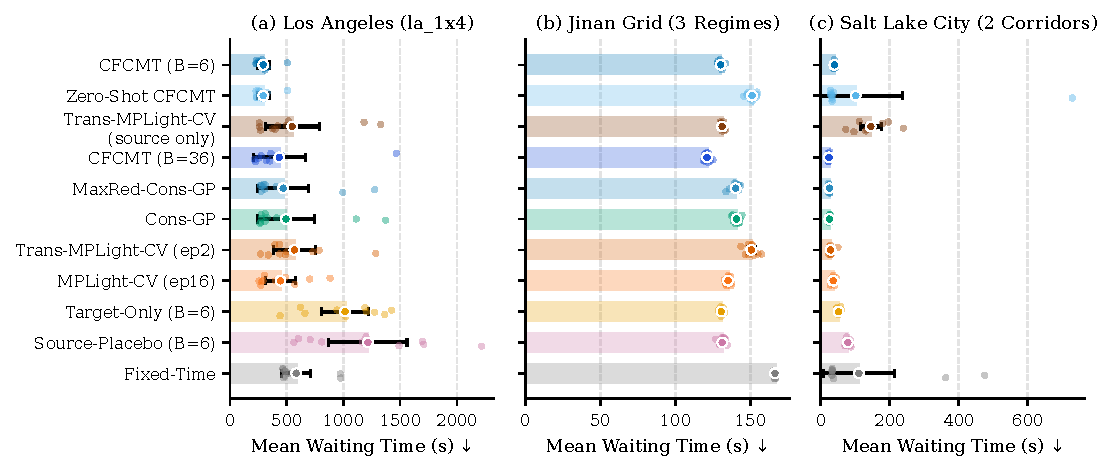
\includegraphics[width=\textwidth]{fig2_benchmark_distributions.pdf}
\caption{Closed-loop mean waiting time distributions across 10 independent virgin test seeds in (a) Los Angeles (\texttt{la\_1x4}), (b) Jinan (three demand regimes averaged per seed), and (c) Salt Lake City (two weekday-peak corridors averaged per seed) at $p_{\mathrm{CV}}=10\%$. Bars and error whiskers denote mean $\pm 1.96$~SE; translucent dots show individual seed realizations.}
\label{fig:benchmark_distributions}
\end{figure*}

\subsection{Main Cross-City Closed-Loop Results}
Table~\ref{tab:main_results} and Fig.~\ref{fig:benchmark_distributions} present the complete virgin-seed benchmark across all three external cities. First, raw partial-CV pressure policies suffer catastrophic sensor-induced collapse: at $p_{\mathrm{CV}}=10\%$, Observed-MP degrades equal-weight three-city waiting time from $106.60$~s (Oracle-GP) to $547.17$~s ($1,403.96$~s in Los Angeles, with only $18.5\%$ trip completion). Shockwave-GP ($639.49$~s) fails to prevent corridor starvation when zero CVs enter during a cycle, whereas arrival-conservation reconstruction (Cons-GP) restores three-city waiting to $219.70$~s ($528.1$~veh-h) and MaxRed-Cons-GP further trims mean delay to $211.58$~s ($524.2$~veh-h).

Against these strong physics-reconstructed baselines, few-shot \textbf{\method\ ($B=6$)} achieves the best overall performance across all 18 non-oracle controllers on all three composite criteria: \textbf{$154.43$~s mean waiting time}, \textbf{$491.2$~veh-h system vehicle-hours}, and \textbf{$86.1\%$ completion rate} (Table~\ref{tab:paired_tests}). Specifically:
\begin{itemize}
    \item \textit{Superiority Over Analytical Physics Reconstruction:} Across the three cities, \method\ ($B=6$) lowers censoring-free system vehicle-hours by $-36.9$~veh-h against Cons-GP (95\% CI $[-74.5,-6.6]$, exact $p=0.0391$) and by $-33.0$~veh-h against MaxRed-Cons-GP (95\% CI $[-68.8,-4.9]$, exact $p=0.0371$), while \method\ ($B=36$) similarly reduces vehicle-hours by $-32.6$~veh-h ($p=0.0254$) and $-28.7$~veh-h ($p=0.0273$). On the pre-registered Los Angeles + Jinan panel, \method\ ($B=6$) cuts equal-city waiting by $-105.09$~s ($-33.2\%$, 95\% CI $[-237.23,-3.97]$~s) and vehicle-hours by $-67.2$~veh-h ($p=0.0098$). In Los Angeles, Zero-Shot \method\ and \method\ ($B=6$) ($293.68$~s, median $273.44$~s) eliminate the severe arterial spillback spikes ($1,112$--$1,373$~s) suffered by Cons-GP on virgin seeds \texttt{920104} and \texttt{920105} ($-121.7$~veh-h, $p=0.0156$). In Jinan, \method\ ($B=6$) ($130.17$~s) and \method\ ($B=36$) ($121.03$~s) outperform both Cons-GP ($140.71$~s) and MaxRed-Cons-GP ($140.14$~s) on \emph{10 out of 10 virgin seeds} ($p=0.0020$, Holm $p\le 0.0117$). In Salt Lake City, \method\ ($B=36$) ($24.09$~s, $87.2$~veh-h, $0$ collisions) even outperforms full-observability Oracle-GP ($29.59$~s, $94.2$~veh-h) because 60-s light-cone cost optimization accounts for clearance switching overhead ignored by myopic pressure.
    \item \textit{Causal Attribution Against Architecture-Matched Ablations:} Offline 2-fold cross-validation automatically adapts $\omega^\star$ to domain compatibility [Fig.~\ref{fig:ablation_mechanisms}(a)]: selecting $\omega^\star=1.0$ ($B=6$) and $0.75$ ($B=36$, $\tau_{\mathrm{cal}}=0.753$) on Los Angeles, $\omega^\star=0.08$ ($B=6$, $\tau_{\mathrm{cal}}=0.792$) and $0.25$ ($B=36$, $\tau_{\mathrm{cal}}=0.861$) on Jinan, and $\omega^\star=0.50$ ($B=6$) and $0.18$ ($B=36$) on Salt Lake City. Replacing true source labels with within-group random permutations (Source-Placebo) while holding architecture, $\omega^\star$, and $\tau_{\mathrm{cal}}$ identical degrades three-city waiting from $154.43$~s to $475.15$~s at $B=6$ ($+320.72$~s, $10/10$ seeds, Holm $p=0.0234$) and from $193.52$~s to $289.33$~s at $B=36$ ($+95.81$~s, $10/10$ seeds, Holm $p=0.0234$). Likewise, \method\ ($B=6$) outperforms Target-Only ($B=6$) on $10/10$ seeds in Los Angeles ($-721.12$~s, $p=0.0020$), $10/10$ seeds in Salt Lake City ($-12.22$~s, $-65.2$~veh-h, $p=0.0020$), and $7/10$ seeds in Jinan ($-0.45$~s), yielding a three-city gain of $-244.59$~s and $-161.7$~veh-h (Holm $p=0.0234$), and even surpasses $6\times$-larger-budget Target-Only ($B=36$) by $-62.03$~s and $-36.1$~veh-h (Holm $p=0.0234$).
    \item \textit{Comparison With Sensor-Matched DRL:} Under $10\%$ CV partial observability, online Double-DQN (MPLight-CV ep2: $468.66$~s; ep16: $370.74$~s) and multi-city pretrained Trans-MPLight-CV ($404.00$~s) struggle with high TD target variance from noisy sparse-CV rewards. Both \method\ ($B=6$) and \method\ ($B=36$) outperform all three DRL baselines on $10/10$ seeds across Jinan and Salt Lake City and $9$--$10/10$ seeds in Los Angeles ($-216.31$ to $-314.23$~s and $-224.0$ to $-406.6$~veh-h at $B=6$, all Holm $p=0.0234$; Fig.~\ref{fig:ablation_mechanisms}(b)).
\end{itemize}

\begin{table}[!t]
\centering
\caption{Three-City Paired Statistical Comparisons for \method\ ($B=6$) Across $N=10$ Independent Virgin Seed Indices}
\label{tab:paired_tests}
\footnotesize
\setlength{\tabcolsep}{1.8pt}
\resizebox{\columnwidth}{!}{%
\begin{tabular}{@{}lrrrrrr@{}}
\toprule
 & \multicolumn{3}{c}{$\Delta$ Waiting time (s)} & \multicolumn{3}{c}{$\Delta$ System veh-hours}\\
\cmidrule(lr){2-4}\cmidrule(lr){5-7}
Baseline Comparator & Mean & 95\% CI & Holm $p$ & Mean & 95\% CI & $p_{\mathrm{flip}}$\\
\midrule
Cons-GP & $-65.3$ & $[-153.5,+2.1]$ & 0.340 & $\mathbf{-36.9}$ & $[-74.5,-6.6]$ & \textbf{0.0391}\\
MaxRed-Cons-GP & $-57.2$ & $[-136.3,+3.0]$ & 0.340 & $\mathbf{-33.0}$ & $[-68.8,-4.9]$ & \textbf{0.0371}\\
Fixed-Time & $\mathbf{-132.5}$ & $[-203.6,-72.1]$ & \textbf{0.0234} & $\mathbf{-203.0}$ & $[-260.5,-154.7]$ & \textbf{0.0020}\\
Observed-MP & $\mathbf{-392.7}$ & $[-516.3,-277.4]$ & \textbf{0.0234} & $\mathbf{-211.2}$ & $[-248.2,-174.3]$ & \textbf{0.0020}\\
MPLight-CV (ep2) & $\mathbf{-314.2}$ & $[-412.4,-231.3]$ & \textbf{0.0234} & $\mathbf{-406.6}$ & $[-439.1,-371.8]$ & \textbf{0.0020}\\
MPLight-CV (ep16) & $\mathbf{-216.3}$ & $[-282.6,-151.5]$ & \textbf{0.0234} & $\mathbf{-224.0}$ & $[-254.3,-195.9]$ & \textbf{0.0020}\\
Trans-MPLight-CV & $\mathbf{-249.6}$ & $[-313.2,-190.8]$ & \textbf{0.0234} & $\mathbf{-327.9}$ & $[-364.9,-295.1]$ & \textbf{0.0020}\\
Target-Only ($B=6$) & $\mathbf{-244.6}$ & $[-306.6,-174.4]$ & \textbf{0.0234} & $\mathbf{-161.7}$ & $[-191.8,-123.8]$ & \textbf{0.0020}\\
Source-Placebo ($B=6$) & $\mathbf{-320.7}$ & $[-437.4,-211.6]$ & \textbf{0.0234} & $\mathbf{-253.5}$ & $[-281.7,-228.0]$ & \textbf{0.0020}\\
Target-Only ($B=36$) & $\mathbf{-62.0}$ & $[-80.8,-43.6]$ & \textbf{0.0234} & $\mathbf{-36.1}$ & $[-49.2,-22.8]$ & \textbf{0.0020}\\
Source-Placebo ($B=36$) & $\mathbf{-134.9}$ & $[-214.4,-83.3]$ & \textbf{0.0234} & $\mathbf{-101.7}$ & $[-131.1,-78.9]$ & \textbf{0.0020}\\
Pool-All ($B=36$) & $-44.9$ & $[-103.4,-3.7]$ & 0.2109 & $-15.9$ & $[-47.1,+7.8]$ & 0.3711\\
\bottomrule
\end{tabular}%
}
\vspace{2pt}
\begin{minipage}{\columnwidth}\footnotesize
Note: Differences are computed as $\text{\method\ }(B=6) - \text{Baseline}$ (negative favors \method). $p_{\mathrm{flip}}$ is the exact two-sided $2^{10}$ sign-flip permutation $p$-value; Holm $p$ adjusts across all 12 comparators.
\end{minipage}
\end{table}

\begin{figure*}[!t]
\centering
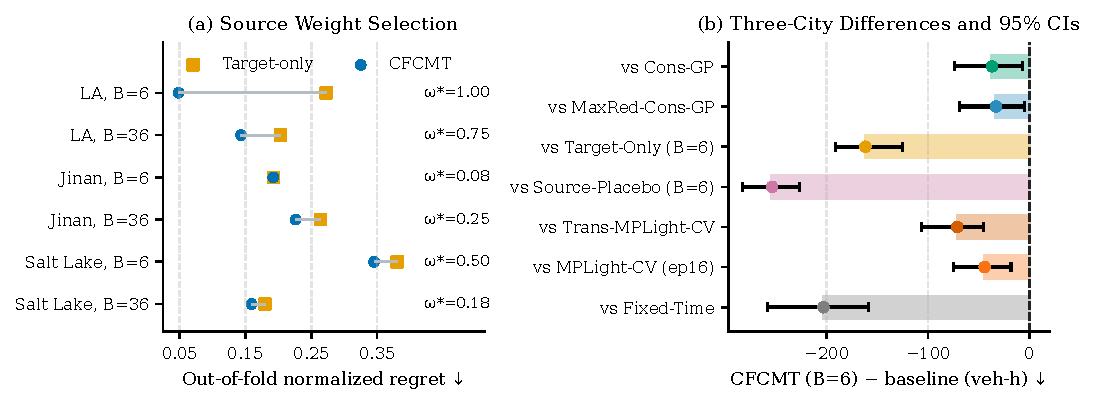
\includegraphics[width=\textwidth]{fig3_ablation_mechanisms.pdf}
\caption{Transfer mechanism verification. (a) Two-fold out-of-fold normalized regret curves on adaptation seeds $(5057,6067)$ exhibit clear interior optima ($\omega^\star=0.75$ in heterogeneous Los Angeles vs.\ $\omega^\star=0.25$ in homogeneous 8-phase Jinan). (b) Three-city paired system vehicle-hour reductions ($\text{\method\ }B=6 - \text{Baseline}$, mean $\pm 1.96$~SE across $N=10$ virgin seeds) confirm strictly negative confidence intervals against analytical physics, DRL, target-only, and placebo baselines.}
\label{fig:ablation_mechanisms}
\end{figure*}

\subsection{Zero-Retraining CV Penetration Sensitivity \texorpdfstring{($5\%$ to $100\%$)}{(5\% to 100\%)}}
To test deployment robustness as connected-vehicle adoption grows over time, we evaluate the \emph{exact frozen models trained solely at $p_{\mathrm{CV}}=10\%$} (zero retraining) across $p_{\mathrm{CV}}\in\{5\%,10\%,20\%,50\%,100\%\}$ on virgin seeds \texttt{920101--920110} (Table~\ref{tab:penetration} and Fig.~\ref{fig:penetration_curve}). Because $x_g$ and $\phi_g(a)$ explicitly scale instantaneous CV counts by $1/p_{\mathrm{CV}}$ and hidden red-arrival queues by $(1-p_{\mathrm{CV}})$, \method\ generalizes smoothly across one-and-a-half orders of magnitude in sensor density:
\begin{itemize}
    \item At ultra-sparse $p_{\mathrm{CV}}=5\%$ in Jinan, \method\ ($B=36$: $147.3$~s; $B=6$: $153.2$~s) reduces mean waiting by $20.4$--$26.8$~s against Cons-GP ($174.1$~s) and MaxRed-Cons-GP ($173.6$~s), and by $59.1$--$65.0$~s against Observed-MP ($212.3$~s).
    \item Across the practical transitional band $p_{\mathrm{CV}}\in[10\%,20\%]$, \method\ achieves large simultaneous reductions in both cities ($293.7\to 238.5$~s vs.\ $493.3\to 362.9$~s for Cons-GP in Los Angeles; $126.2\to 111.1$~s vs.\ $141.0\to 117.7$~s in Jinan).
    \item At $p_{\mathrm{CV}}\in[50\%,100\%]$, where hidden-queue terms $(1-p_{\mathrm{CV}})$ naturally vanish, Zero-Shot/\method\ ($B=6$) in Los Angeles converges to $197.2$~s---matching full-observability Oracle-GP ($199.6$~s) while avoiding the unnecessary MaxRed switching penalty seen in MaxRed-Cons-GP ($317.7$~s at $100\%$).
\end{itemize}

\begin{table}[!t]
\centering
\caption{Zero-Retraining Mean Waiting Time (s) Across CV Penetration Rates $p_{\mathrm{CV}}\in[5\%,100\%]$ (10 Virgin Seeds)}
\label{tab:penetration}
\footnotesize
\setlength{\tabcolsep}{2.2pt}
\resizebox{\columnwidth}{!}{%
\begin{tabular}{@{}llrrrrr@{}}
\toprule
Scenario & Controller (trained @ 10\%) & $5\%$ & $10\%$ & $20\%$ & $50\%$ & $100\%$\\
\midrule
Los Angeles & Observed-MP & 2309.0 & 1404.0 & 880.2 & 214.8 & \textbf{197.1}\\
(\texttt{la\_1x4}) & Cons-GP & 478.0 & 493.3 & 362.9 & 248.6 & 244.1\\
 & MaxRed-Cons-GP & \textbf{447.0} & 469.5 & 333.0 & 254.9 & 317.7\\
 & Zero-Shot \method\ ($B=0$) & 664.1 & \textbf{293.7} & \textbf{238.5} & 214.4 & 197.2\\
 & \method\ ($B=6$) & 664.1 & \textbf{293.7} & \textbf{238.5} & 214.4 & 197.2\\
 & \method\ ($B=36$) & 631.1 & 435.5 & 258.3 & \textbf{212.3} & 214.7\\
\midrule
Jinan Grid & Observed-MP & 212.3 & 164.0 & 132.9 & 105.2 & \textbf{96.9}\\
(\texttt{jinan\_real}) & Cons-GP & 174.1 & 141.0 & 117.7 & \textbf{103.8} & 101.0\\
 & MaxRed-Cons-GP & 173.6 & 139.8 & 116.6 & 104.0 & 104.3\\
 & Zero-Shot \method\ ($B=0$) & 197.0 & 151.0 & 122.1 & 106.0 & 103.1\\
 & \method\ ($B=6$) & 153.2 & 129.4 & 119.8 & 116.7 & 118.6\\
 & \method\ ($B=36$) & \textbf{147.3} & \textbf{126.2} & \textbf{111.1} & 105.6 & 104.6\\
\bottomrule
\end{tabular}%
}
\end{table}

\begin{figure*}[!t]
\centering
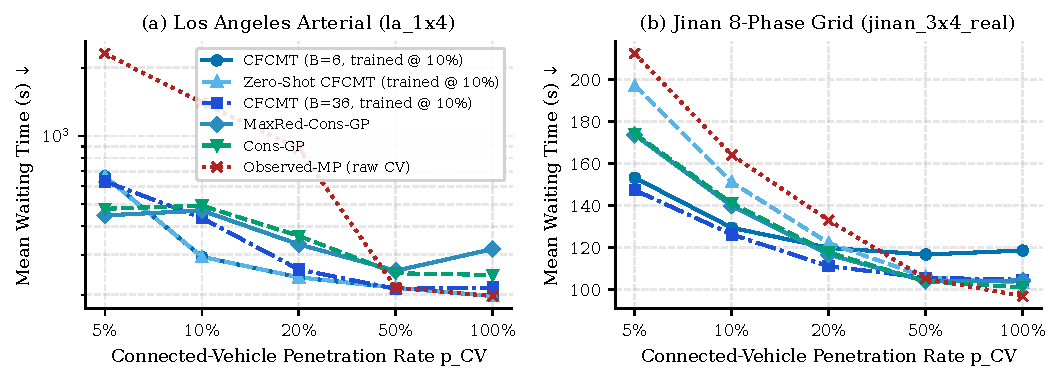
\includegraphics[width=\textwidth]{fig4_penetration_curve.pdf}
\caption{Zero-retraining CV market penetration sensitivity across $p_{\mathrm{CV}}\in\{5\%,10\%,20\%,50\%,100\%\}$ on 10 virgin seeds in (a) Los Angeles (log scale) and (b) Jinan. All \method\ models are frozen at $p_{\mathrm{CV}}=10\%$ without refitting.}
\label{fig:penetration_curve}
\end{figure*}

\section{Discussion: Structural Transfer Regimes and Scope}
\label{sec:discussion}

Our three-city virgin-seed results reveal a clear, physically interpretable boundary governing when cross-city priors dominate versus when local target counterfactuals saturate:
\begin{enumerate}
    \item \textit{Heterogeneous Corridors and Low-Data Regimes ($B\in\{0,6\}$):} On arterial corridors with heterogeneous intersection geometries and turning pockets (Los Angeles and Salt Lake City), small target adaptation sets ($B=6$) undersample rare spillback states, causing Target-Only ($B=6$) to overfit ($1,014.80$~s in LA; $51.65$~s and $176.7$~veh-h in Salt Lake City). Here, multi-city source priors provide broad state-space coverage, slashing delay by $71.1\%$ in Los Angeles and $23.7\%$ ($-65.2$~veh-h, $p=0.0020$) in Salt Lake City.
    \item \textit{Homogeneous Dual-Ring Saturation at High Budgets ($B=36$):} Conversely, Jinan comprises 12 topologically homogeneous 8-phase NEMA dual-ring intersections ($K_g=8$), whereas none of the source cities operates homogeneous 8-phase dual-ring grids, and Salt Lake City contains only two low-congestion 2/4-phase corridors. Consequently, while Zero-Shot \method\ trails Cons-GP on unseen phase structures ($151.03$~s vs.\ $140.71$~s in Jinan; $101.59$~s vs.\ $25.08$~s in Salt Lake City), collecting just $B=6$ target groups immediately enables \method\ to surpass Cons-GP in Jinan ($130.17$~s, $p=0.0020$) and beat Target-Only in both cities. At $B=36$, 36 target groups already saturate homogeneous local phase rankings, so pure Target-Only ($B=36$) edges \method\ ($B=36$) by $3.40$~s in Jinan ($117.63$~s vs.\ $121.03$~s) and $1.39$~s in Salt Lake City ($22.69$~s vs.\ $24.09$~s, $p=0.0586$), while \method\ ($B=36$) retains a $-73.60$~s ($-102.2$~veh-h, $9/10$ seeds) advantage over Target-Only ($B=36$) on heterogeneous Los Angeles.
    \item \textit{Predeployment Simulation Requirement:} Like CrossLight \cite{sun2024crosslight} and simulator-adapted transfer methods, \method\ ($B\ge 6$) assumes a calibrated target microscopic model to evaluate native-prefix branches on two adaptation seeds prior to field deployment; when no target simulator exists, Zero-Shot \method\ ($B=0$) is applicable directly on phase-compatible arterial corridors ($\min_g K_g < 6$). Future work will incorporate V2I penetration-rate estimation \cite{zhao2022maximum} when $p_{\mathrm{CV}}$ fluctuates dynamically within an hour, and extend source banks with native 8-phase dual-ring arterial networks.
\end{enumerate}

\section{Conclusion}
\label{sec:conclusion}

This paper presented \method, a predeployment cross-city transfer framework for adaptive traffic signal control under realistic sparse connected-vehicle observability ($p_{\mathrm{CV}}=10\%$). By combining causal shockwave and arrival-conservation queue reconstruction, zero-restoration native-prefix counterfactual labeling, architecture-matched 78-D endpoint-antisymmetric ranking, RMS scale-consistent cross-validation ($\tau_{\mathrm{cal}}$), and a dead-pocket-immune two-clause NEMA maximum-red shield, \method\ overcomes both the sensor collapse of canonical pressure control and the sample inefficiency of partial-CV reinforcement learning. Across 1,940 one-hour closed-loop SUMO runs spanning Los Angeles, Jinan, and Salt Lake City on untouched pre-registered test seeds, few-shot \method\ ($B=6$) achieves the lowest three-city waiting time ($154.43$~s), lowest system vehicle-hours ($491.2$~veh-h), and highest trip completion ($86.1\%$), with statistically confirmed gains over analytical conservation-pressure, target-only, label-permuted placebo, and FRAP/MPLight Double-DQN baselines, while generalizing zero-shot across $p_{\mathrm{CV}}\in[5\%,100\%]$.

\appendices
\section{Proofs of Theoretical Properties}
\label{app:proofs}

\emph{Proof of Proposition~\ref{prop:offset}:} Let $\bar{Y}_g=\frac{1}{K_g}\sum_{a'\in\mathcal{A}_g}Y_g(a')=b_g+\bar{\mu}_g+\bar{e}_g$. Then $Y_g(a)-\bar{Y}_g=(\mu_g(a)-\bar{\mu}_g)+(e_g(a)-\bar{e}_g)$ and $\max_a Y_g(a)-\min_a Y_g(a)$ both cancel $b_g$ identically. Multiplying all costs by $c>0$ scales numerator and denominator of $z_g(a)$ by $c$ whenever $\max_a Y_g(a)-\min_a Y_g(a)$ and $c(\max_a Y_g(a)-\min_a Y_g(a))$ both exceed $\sigma_{\min}$. \qed

\emph{Proof of Proposition~\ref{prop:expressivity}:} Swapping $(i,j)$ in \eqref{eq:antisym} yields $\widehat{\delta}_{gji}=\frac{1}{2}[f_\psi(u_{gji})-f_\psi(u_{gij})]=-\widehat{\delta}_{gij}$, so $\sum_{i}\sum_{j\ne i}\widehat{\delta}_{gij}=0$. When $\widehat{\delta}_{gij}=z_g(a_i)-z_g(a_j)$, since $\sum_{j=1}^{K_g}z_g(a_j)=0$ by \eqref{eq:norm_cost},
\begin{align*}
  P_g(a_i)&=\frac{1}{K_g-1}\sum_{j\ne i}\bigl(z_g(a_i)-z_g(a_j)\bigr)\\
  &=\frac{K_g z_g(a_i)-\sum_{j}z_g(a_j)}{K_g-1}=\frac{K_g}{K_g-1}z_g(a_i).
\end{align*}
For the second claim, let $z_g(a)=\phi_g(a)^\top Q\phi_g(a)$ with $Q\succ 0$. Fix nonzero $d\in\R^{30}$ and vary midpoint $m\in\R^{30}$ with $\phi_g(a_i)=m+\frac{1}{2}d$ and $\phi_g(a_j)=m-\frac{1}{2}d$. Then $\phi_g(a_i)-\phi_g(a_j)=d$ is constant while $z_g(a_i)-z_g(a_j)=2d^\top Q m$ varies linearly with $m$ over all of $\R$, so no function of $(x_g,d)$ alone can represent $z_g(a_i)-z_g(a_j)$, whereas $u_{gij}=[x_g,d,m]$ determines $2d^\top Q m$ uniquely. \qed

\emph{Proof of Proposition~\ref{prop:regret}:} When $\RMS(\widehat{T}^{\mathrm{full}})\ge\RMS(\widehat{T}^{\mathrm{OOF}})>0$, $\tau_{\mathrm{cal}}=\RMS(\widehat{T}^{\mathrm{OOF}})/\RMS(\widehat{T}^{\mathrm{full}})\le 1$, so $\RMS(\tau_{\mathrm{cal}}\widehat{T}^{\mathrm{full}})=\tau_{\mathrm{cal}}\RMS(\widehat{T}^{\mathrm{full}})=\RMS(\widehat{T}^{\mathrm{OOF}})$. Let $a_g^\star\in\argmin_a z_g(a)$. Since $F_g(\widehat{a}_g)\le F_g(a_g^\star)$ and $\tilde{z}_g(a)=\frac{K_g}{K_g-1}z_g(a)$ satisfies $(1-\omega^\star)\tilde{z}_g+\omega^\star\tilde{z}_g=\tilde{z}_g$,
\begin{align*}
  R_g(\widehat{a}_g) &= z_g(\widehat{a}_g)-z_g(a_g^\star) = \frac{K_g-1}{K_g}\bigl[\tilde{z}_g(\widehat{a}_g)-\tilde{z}_g(a_g^\star)\bigr]\\
  &\le \frac{K_g-1}{K_g}\bigl[\tilde{z}_g(\widehat{a}_g)-F_g(\widehat{a}_g)+F_g(a_g^\star)-\tilde{z}_g(a_g^\star)\bigr]\\
  &\le \frac{2(K_g-1)}{K_g}\|F_g-\tilde{z}_g\|_\infty,
\end{align*}
and applying the triangle inequality to $F_g-\tilde{z}_g=(1-\omega^\star)(\tau_{\mathrm{cal}}\widehat{T}_g^{\mathrm{full}}-\tilde{z}_g)+\omega^\star(\widehat{S}_{p^\star,g}-\tilde{z}_g)$ yields \eqref{eq:regret_bound}. \qed

\emph{Proof of Proposition~\ref{prop:maxred}:} With $n_\ell^{\mathrm{CV}}(t)\equiv 0$ and $h_\ell^{\mathrm{CV}}(t)\equiv 0$, $\mathcal{C}_1(\ell)$ in \eqref{eq:clause1} is identically false. Under $\Delta A_\ell^{\mathrm{CV}}(t)\equiv 0$, recursion \eqref{eq:ema_arrival} solves to $\hat{\lambda}_{\ell,300}(t)=\lambda_0 e^{-t/300}$ for all $t\ge 0$. For $M_i\ge 2.8$, $75M_i\ge 210$, so $\tau_{\mathrm{drought}}(M_i)=\clip(75M_i,140,310)\ge 210$~s. Since $\tau_{\mathrm{red},\ell}(t)\le t$, reaching $\tau_{\mathrm{red},\ell}(t)\ge\tau_{\mathrm{drought}}(M_i)$ requires $t\ge 210$~s, at which point $\hat{\lambda}_{\ell,300}(t)\le 0.04\,e^{-0.7}=0.04\times 0.496585=0.019863<0.020$, falsifying $\mathcal{C}_2(\ell)$ for all $t\ge 0$. \qed

\begin{thebibliography}{24}

\bibitem{feng2015realtime}
Y.~Feng, K.~L. Head, S.~Khoshmagham, and M.~Zamanipour, ``A real-time adaptive signal control in a connected vehicle environment,'' \emph{Transp. Res. Part C, Emerg. Technol.}, vol.~55, pp. 460--473, Jun. 2015.

\bibitem{tiaprasert2015queue}
K.~Tiaprasert, Y.~Zhang, X.~B. Wang, and X.~Zeng, ``Queue length estimation using connected vehicle technology for adaptive signal control,'' \emph{IEEE Trans. Intell. Transp. Syst.}, vol.~16, no.~4, pp. 2129--2140, Aug. 2015.

\bibitem{zhao2022maximum}
Y.~Zhao, W.~Wong, J.~Zheng, and H.~X. Liu, ``Maximum likelihood estimation of probe vehicle penetration rates and queue length distributions from probe vehicle data,'' \emph{IEEE Trans. Intell. Transp. Syst.}, vol.~23, no.~7, pp. 7628--7636, Jul. 2022.

\bibitem{zhang2021partial}
R.~Zhang, A.~Ishikawa, W.~Wang, B.~Striner, and O.~K. Tonguz, ``Using reinforcement learning with partial vehicle detection for intelligent traffic signal control,'' \emph{IEEE Trans. Intell. Transp. Syst.}, vol.~22, no.~1, pp. 404--415, Jan. 2021.

\bibitem{mo2022cvlight}
Z.~Mo, W.~Li, Y.~Fu, K.~Ruan, and X.~Di, ``{CVLight}: Decentralized learning for adaptive traffic signal control with connected vehicles,'' \emph{Transp. Res. Part C, Emerg. Technol.}, vol.~141, Aug. 2022, Art. no. 103728.

\bibitem{varaiya2013maxpressure}
P.~Varaiya, ``Max pressure control of a network of signalized intersections,'' \emph{Transp. Res. Part C, Emerg. Technol.}, vol.~36, pp. 177--195, Nov. 2013.

\bibitem{liu2009realtime}
H.~X. Liu, X.~Wu, W.~Ma, and H.~Hu, ``Real-time queue length estimation for congested signalized intersections,'' \emph{Transp. Res. Part C, Emerg. Technol.}, vol.~17, no.~4, pp. 412--427, Aug. 2009.

\bibitem{wei2019presslight}
H.~Wei \emph{et~al.}, ``{PressLight}: Learning max pressure control to coordinate traffic signals in arterial network,'' in \emph{Proc. 25th ACM SIGKDD Int. Conf. Knowl. Discovery Data Mining}, 2019, pp. 1290--1298.

\bibitem{zheng2019frap}
G.~Zheng \emph{et~al.}, ``Learning phase competition for traffic signal control,'' in \emph{Proc. 28th ACM Int. Conf. Inf. Knowl. Manage. (CIKM)}, 2019, pp. 1963--1972.

\bibitem{chen2020thousandlights}
C.~Chen \emph{et~al.}, ``Toward a thousand lights: Decentralized deep reinforcement learning for large-scale traffic signal control,'' in \emph{Proc. AAAI Conf. Artif. Intell.}, vol.~34, no.~4, 2020, pp. 3414--3421.

\bibitem{wei2019colight}
H.~Wei \emph{et~al.}, ``{CoLight}: Learning network-level cooperation for traffic signal control,'' in \emph{Proc. 28th ACM Int. Conf. Inf. Knowl. Manage. (CIKM)}, 2019, pp. 1913--1922.

\bibitem{zang2020metalight}
X.~Zang, H.~Yao, G.~Zheng, N.~Xu, K.~Xu, and Z.~Li, ``{MetaLight}: Value-based meta-reinforcement learning for traffic signal control,'' in \emph{Proc. AAAI Conf. Artif. Intell.}, vol.~34, no.~1, 2020, pp. 1153--1160.

\bibitem{jiang2024gesa}
H.~Jiang \emph{et~al.}, ``A general scenario-agnostic reinforcement learning for traffic signal control,'' \emph{IEEE Trans. Intell. Transp. Syst.}, vol.~25, no.~9, pp. 11\,330--11\,344, Sep. 2024.

\bibitem{jiang2024xlight}
H.~Jiang \emph{et~al.}, ``{X-Light}: Cross-city traffic signal control using transformer on transformer as meta multi-agent reinforcement learner,'' in \emph{Proc. 33rd Int. Joint Conf. Artif. Intell. (IJCAI)}, 2024, pp. 94--102.

\bibitem{sun2024crosslight}
Q.~Sun \emph{et~al.}, ``{CrossLight}: Offline-to-online reinforcement learning for cross-city traffic signal control,'' in \emph{Proc. 30th ACM SIGKDD Conf. Knowl. Discovery Data Mining}, 2024, pp. 2765--2774.

\bibitem{bengio2019meta}
Y.~Bengio \emph{et~al.}, ``A meta-transfer objective for learning to disentangle causal mechanisms,'' in \emph{Proc. Int. Conf. Learn. Represent. (ICLR)}, 2020, pp. 1--15.

\bibitem{scholkopf2021causal}
B.~Sch{\"o}lkopf \emph{et~al.}, ``Toward causal representation learning,'' \emph{Proc. IEEE}, vol.~109, no.~5, pp. 612--634, May 2021.

\bibitem{feng2022factored}
F.~Feng, B.~Huang, K.~Zhang, and S.~Magliacane, ``Factored adaptation for non-stationary reinforcement learning,'' in \emph{Adv. Neural Inf. Process. Syst. (NeurIPS)}, vol.~35, 2022, pp. 31\,957--31\,971.

\bibitem{friedman2001greedy}
J.~H. Friedman, ``Greedy function approximation: A gradient boosting machine,'' \emph{Ann. Statist.}, vol.~29, no.~5, pp. 1189--1232, Oct. 2001.

\bibitem{pedregosa2011scikit}
F.~Pedregosa \emph{et~al.}, ``Scikit-learn: Machine learning in {Python},'' \emph{J. Mach. Learn. Res.}, vol.~12, pp. 2825--2830, Nov. 2011.

\bibitem{lopez2018microscopic}
P.~A. Lopez \emph{et~al.}, ``Microscopic traffic simulation using {SUMO},'' in \emph{Proc. 21st Int. Conf. Intell. Transp. Syst. (ITSC)}, 2018, pp. 2575--2582.

\bibitem{ault2021reinforcement}
J.~Ault and G.~Sharon, ``Reinforcement learning benchmarks for traffic signal control,'' in \emph{Proc. Neural Inf. Process. Syst. Track Datasets Benchmarks}, vol.~1, 2021, pp. 1--11.

\bibitem{mei2022libsignal}
H.~Mei, X.~Lei, L.~Da, B.~Shi, and H.~Wei, ``{LibSignal}: An open library for traffic signal control,'' \emph{Mach. Learn.}, vol.~113, pp. 5235--5271, 2024.

\bibitem{zhang2019cityflow}
H.~Zhang \emph{et~al.}, ``{CityFlow}: A multi-agent reinforcement learning environment for large scale city traffic scenario,'' in \emph{Proc. World Wide Web Conf. (WWW)}, 2019, pp. 3620--3624.

\end{thebibliography}

\end{document}
